
\chapter{موارد کاربرد}


\section{تعریف کنش‌گر‌ها}


\begin{table}[h]
	\setlength\extrarowheight{-5pt}
	\centering
	\begin{tabular}{|p{0.05\linewidth}|p{0.15\linewidth}|p{0.75\linewidth}|} 
\hline
\multicolumn{1}{|c|}{\textbf{ردیف}} & \textbf{نام}  & \multicolumn{1}{c|}{\textbf{توضیح}}                                                                                                                                  \\ \hline
۱                                   & مشتری         & نقشی که در سامانه درخواست خدمت می‌کند.                                                                                                                               \\ \hline
۲                                   & متخصص         & نقشی که دارای یک یا چند تخصص است و به خدمات درخواست شده در سامانه رسیدگی می‌کند.                                                                                     \\ \hline
۳                                   & مدیر شرکت     & نقشی با بالاترین سطح دسترسی و دید کسب‌و‌کاری که امکان ویرایش اطلاعات را دارد و همچنین گزارش‌های آماری از انجام کارها در سیستم را دریافت و بر کار سیستم نظارت می‌کند. \\ \hline
۴                                   & مدیر فنی شرکت & نقشی که بررسی مشکلات فنی سیستم را برعهده دارد.  
 \\ \hline

	\end{tabular}
\end{table}
\newpage
\section{نمودار موارد کاربرد}


\begin{figure}[ht!]
\centering
		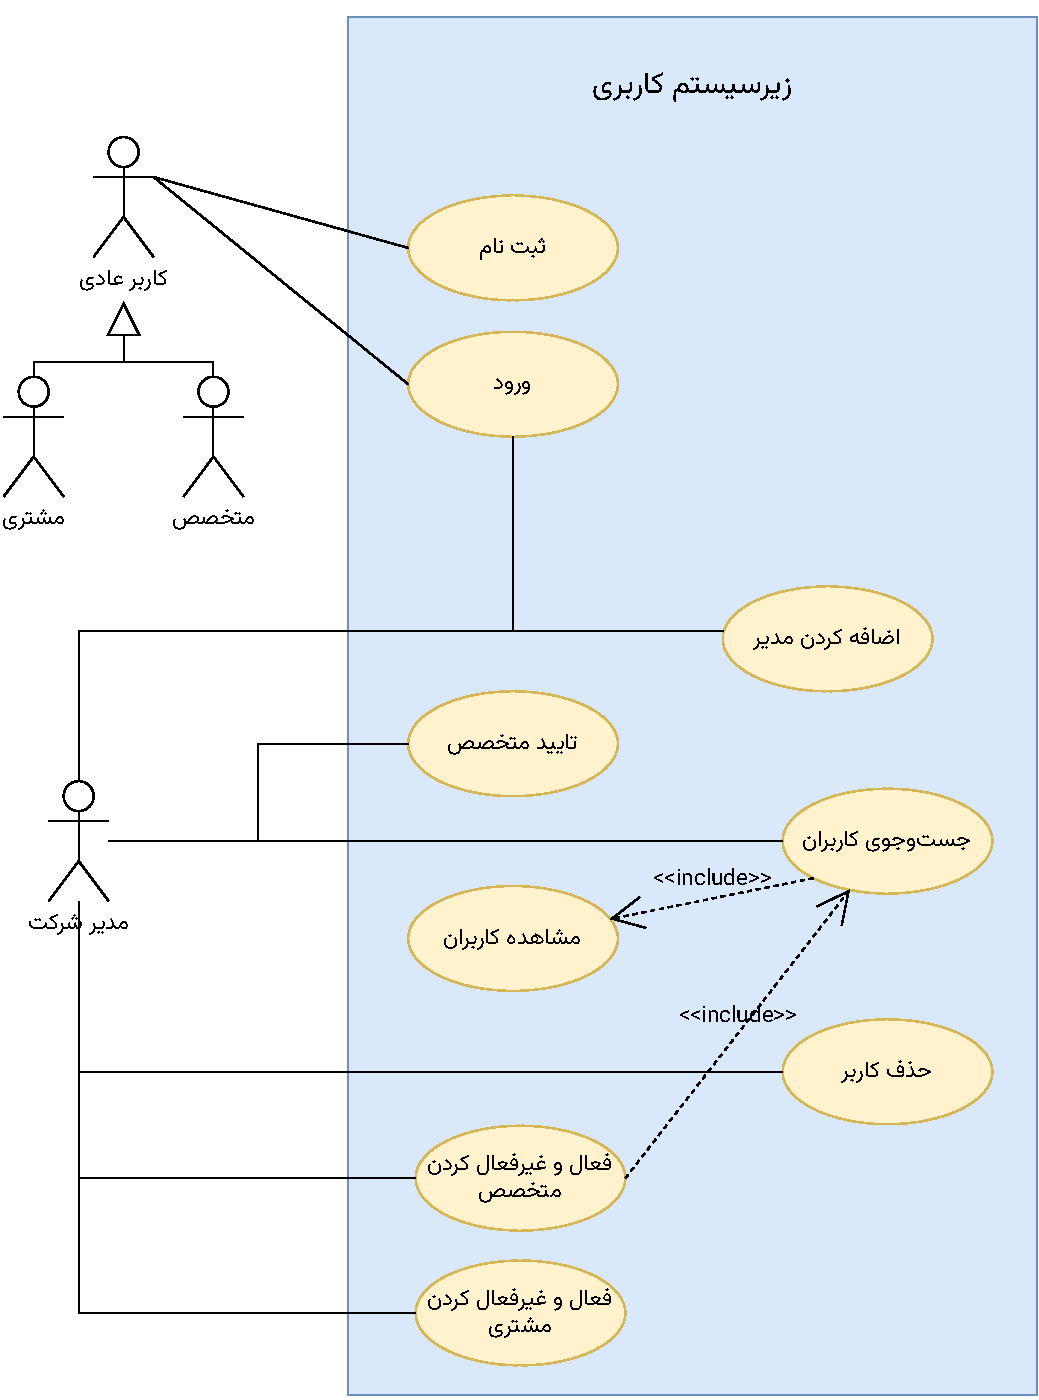
\includegraphics[scale=0.8, page=1]{figs/usecase.pdf}
\caption{زیرسیستم کاربری}
\end{figure}

\FloatBarrier
\newpage


\begin{figure}
\centering
	\includegraphics[scale=0.9, page=2]{figs/usecase.pdf}
\caption{زیرسیستم خدمت‌دهی}
\end{figure}
\FloatBarrier
\newpage

\begin{figure}
\centering
	\includegraphics[scale=0.9, page=3]{figs/usecase.pdf}
\caption{زیرسیستم بازخورد}
\end{figure}
\FloatBarrier
\newpage

\begin{figure}
\centering
	\includegraphics[scale=0.9, page=4]{figs/usecase.pdf}
\caption{زیرسیستم گزارش‌گیری}
\end{figure}
\FloatBarrier
\newpage

\newpage
\section{فهرست موارد کاربرد}


\subsection{زیرسیستم کاربری}
\renewcommand{\labelenumiii}{\arabic{enumi}.\arabic{enumii}.\arabic{enumiii}}
\usecase
{ثبت نام}
{۱}
{مشتری یا متخصص، در سایت ثبت نام می‌کنند تا بتوانند از امکانات سایت استفاده کنند.}
{مشتری، متخصص}
{}{کاربر (مشتری یا متخصص) وارد حساب کاربری خود نشده باشد (لاگین نکرده باشد).}
{
\vspace*{-0.6cm}
\begin{enumerate}
	\item 
	کاربر اقدام به ثبت نام در سایت به عنوان متخصص یا مشتری می‌کند.
	\item
	\textbf{تا زمانی که} اطلاعات کاربر به طور کامل وارد نشده است:
	
	\begin{enumerate}[label=\theenumi.\arabic*.]
	\item
	کاربر اطلاعات هویتی شامل نام و نام‌خانوادگی و همچنین شماره تلفن همراه و ایمیل را وارد می‌کند.
	\item 
	کاربر رمز عبور خود را وارد می‌کند.
	
	\item 
	\textbf{اگر} کاربر قصد ثبت نام به عنوان متخصص را داشت:
	\begin{enumerate}
		\item 
		کاربر تخصص‌هایی که در آن‌ها مهارت دارد را وارد می‌کند.
	\end{enumerate}

	\item 
	کاربر اطلاعات خود را ثبت می‌کند.
	
	\item 
	سیستم صحت کلی اطلاعات کاربر را کنترل می‌کند.
	\end{enumerate}
	
	\item 
	سیستم ثبت‌نام موفق را به اطلاع کاربر می‌رساند.
	
	
\end{enumerate}
}
{یک اکانت برای کاربر ساخته می‌شود. در صورتی که کاربر به عنوان متخصص ثبت‌نام کرده باشد، در وضعیت در انتظار تایید توسط مدیر قرار می‌گیرد.}
{\begin{itemize}
		\vspace*{-0.6cm}
		\item انصراف: در صورت انصراف، ثبت نام کاربر لغو می‌شود
		\item معتبر نبودن ایمیل در مرحله ۲.۱.: در این صورت سیستم در قالب پیامی کاربر را مطلع می‌کند.
		
		
\end{itemize}}
{مورد کاربرد: ثبت نام}



\alternativeflow
% name
{
	ثبت‌ نام:معتبر نبودن ایمیل
}
% id
{۱.۱}
% brief description
{
	اگر کاربر در حین ثبت‌نام ایمیل نامعتبر وارد کرده باشد، پیام خطا می‌گیرد.
}
% primary actos
{
	مشتری یا متخصص
}
% secondary actors
{}
% preconditons
{
	\begin{itemize}
	
		\item
		کاربر ایمیل نامعتبر وارد کرده باشد..
	\end{itemize}
}
% main flow
{
	\vspace*{-0.6cm}
	\begin{enumerate}
		\item 
		روند جایگزین در مرحله ۲.۱ روند اصلی اتفاق می‌افتد.
		\item
		کاربر ایمیل نامعتبری وارد می‌کند.
		\item 
		سیستم خطای ایمیل نامعتبر را نمایش می‌دهد.
	\end{enumerate}
}
% postconditions
{
	نمایش خطای ایمیل نامعتبر به کاربر
}
% table name
{
	روند جایگزین: 	ثبت‌ نام:معتبر نبودن ایمیل
}




\usecase
{ورود}
{۲}
{کاربرانی که در سایت ثبت‌ نام کرده‌اند یا از ابتدا اکانت دارند (شامل مدیر، مشتری و متخصص) وارد حساب کاربری خود می‌شوند.}
{همه کاربران (مدیر، مشتری و متخصص)}
{}
{
		\begin{itemize}
		\item
		کاربر در سیستم لاگین نکرده باشد.
		\item
		اکانتی برای کاربر در سایت وجود داشته باشد.
	\end{itemize}
	
}
{
\begin{enumerate}
	\item 
	کاربر درخواست وارد شدن به حساب کاربری خود را می‌کند.
	
	
	\item 
	کاربر ایمیل و پسورد خود را وارد می‌کند.
	
	\item
	سیستم درستی اطلاعات وارد شده را بررسی می‌کند.
	
	\item
	کاربر احراز هویت شده و وارد حساب کاربری خود می‌شود.
\end{enumerate}
}{اگر اطلاعات وارد شده درست باشد، کاربر وارد حساب کاربری خود می‌شود.}
{	
	
	\begin{itemize}
	\item
	 انصراف: در صورت انصراف، ورود کاربر لغو می‌شود.
	
	\item
	اشتباه بودن اطلاعات وارد شده: اگر در مرحله ۳ سیستم متوجه اشتباه بودن اطلاعات کاربر شود، با صادر کردن اخطار این موضوع را به کاربر اطلاع می‌دهد. کاربر به مرحله ۲ باز می‌گردد.
	\end{itemize}
}
{مورد کاربرد: ورود }



\alternativeflow
% name
{
	ورود:اشتباه بودن اطلاعات وارد شده
}
% id
{1.2}
% brief description
{
	اگر کاربر در حین ورود اطلاعات اشتباه وارد کند، پیام خطا گرفته و به ابتدای فرآیند ورود باز می گردد
}
% primary actos
{
	مشتری یا متخصص
}
% secondary actors
{}
% preconditons
{
	\begin{itemize}
		
		\item
		اطلاعات ورودی کاربر نادرست باشد.
	\end{itemize}
}
% main flow
{
	\vspace*{-0.6cm}
	\begin{enumerate}
		\item 
		روند جایگزین در مرحله ۳ روند اصلی اتفاق می‌افتد.
		\item
		کاربر اطلاعات ورود نادرستی وارد می‌کند.
		\item 
		سیستم خطای اطلاعات نامعتبر را نمایش می‌دهد.
		\item
		کاربر به مرحله ۲ روند اصلی باز می‌گردد.
	\end{enumerate}
}
% postconditions
{
	بازگشت کاربر به مرحله ۲ از روند اصلی
}
% table name
{
	روند جایگزین: ورود:اشتباه بودن اطلاعات وارد شده
}


\usecase
{جست‌وجوی کاربران}
{۳}
{مدیر شرکت با وارد کردن فیلترهای مختلف به جست‌و‌جوی کاربران می‌پردازد}
{مدیر شرکت}
{}
{
	\begin{itemize}
	\item
	مدیر در سیستم لاگین کرده باشد.
	
	\end{itemize}
 }
{
\begin{enumerate}
	\item 
	مدیر وارد قسمت جست‌وجوی کاربران می‌شود.
	
	\item 
	مدیر اطلاعات لازم برای فیلتر‌های جست‌وجو - شامل نام،‌ نام‌خانوادگی، نوع کاربر (متخصص یا مشتری)، تخصص‌ها در صورت انتخاب نوع متخصص، ایمیل و شماره تلفن- را وارد می‌کند.
	
	\item
	سیستم براساس فیلتر‌های وارد شده در لیست کاربران جست‌وجو می‌کند.
	
	\item 
	کاربرانی که با فیلتر‌های وارد شده تطابق داشته باشند، به عنوان خروجی داده می‌شوند.
	
	\item
	شامل (\lr{Include}) مورد کاربری «مشاهده کاربران»
\end{enumerate}
}
{}
{
\begin{itemize}
	\item	
	انصراف: مدیر از حالت جست‌وجوی کاربران خارج می شود.
	
	\item 
	پیدا نشدن هیچ کاربری در مرحله ۳: خطایی در مورد یافت نشدن کاربری با مشخصات وارد شده نمایش داده می‌شود.
\end{itemize}
}
{مورد کاربرد: جست‌وجوی کاربران}


\alternativeflow
% name
{
	جست‌وجوی کاربران:پیدا نشدن هیچ کاربری
}
% id
{1.3}
% brief description
{
	هیچ کاربری با اطلاعات وارد شده یافت نمی‌شود.
}
% primary actos
{
	مدیر شرکت
}
% secondary actors
{}
% preconditons
{
	\begin{itemize}
		
		\item
		هیچ کاربری با اطلاعات وارد شده وجود نداشته باشد.
	\end{itemize}
}
% main flow
{
	\vspace*{-0.6cm}
	\begin{enumerate}
		\item 
		روند جایگزین در مرحله ۳ روند اصلی اتفاق می‌افتد.
		\item
		هیچ کاربری با اطلاعات وارد شده یافت نمی‌شود.
		\item 
		سیستم خطای یافت نشدن کاربری با اطلاعات وارد شده را نمایش می‌دهد.
		\item
	\end{enumerate}
}
% postconditions
{
	پیام خطای وارد نشدن کاربر نمایش داده می‌شود.
}
% table name
{
	روند جایگزین: جست‌وجوی کاربران:پیدا نشدن هیچ کاربری
}



\usecase
{مشاهده کاربران}
{۴}
{مدیر شرکت اطلاعات کاربران مشخص شده را مشاهده می‌کند.}
{مدیر شرکت}
{}
{
		\begin{itemize}
		\item
		مدیر در سیستم لاگین کرده باشد.
		
		\item
		‌کاربرانی که قرار است نمایش داده شوند مشخص شده باشند.
	\end{itemize}
}
{
\begin{enumerate}
	\item 
	سیستم لیست (آی‌دی) کاربرانی که قرار است نمایش داده شوند را دریافت می‌کند.
	
	\item
	سیستم کاربران مشخص شده را به همراه تمامی صفات آنان به مدیر نمایش می‌دهد.
\end{enumerate}
}
{
}
{
	\begin{itemize}
		\item 
		وجود نداشتن برخی از آی‌دی‌های مشخص شده: سیستم اطلاعات کاربری که وجود ندارد را نمایش نمی‌دهد و آن را نادیده می‌گیرد.
	\end{itemize}
}
{مورد کاربرد: مشاهده کاربران}


\usecase
{تایید متخصص}
{۵}
{مدیر شرکت متخصصی که ثبت نام کرده است را تایید یا رد می‌کند}
{مدیر شرکت}
{}
{
	\begin{itemize}
	\item 
	کاربر متخصص در سیستم ثبت‌نام کرده باشد و هنوز تایید نشده باشد.
	
	\item
مدیر در سیستم لاگین کرده باشد.
\end{itemize}
}
{
\begin{enumerate}
	\item 
	شامل (\lr{Include}) مورد کاربری «جست‌وجوی کاربران»
	\item
	سیستم لیست متخصصانی که تایید نشده‌اند را نمایش می‌دهد.
	
	\item 
	مدیر شرکت متخصصی که قصد تایید یا رد آن را دارد انتخاب می‌کند.
	
	\item 
	مدیر شرکت بسته به اطلاعات متخصص، رد یا تایید متخصص را مشخص می‌کند.
\end{enumerate}
}
{\begin{itemize}
	\item
	وضعیت متخصص بسته به انتخاب مدیر، به حالت رد شده یا تایید شده در می‌آید.
\end{itemize}}
{
\begin{itemize}
	\item انصراف: مدیر از قسمت تایید متخصص خارج می‌شود.
\end{itemize}
}
{مورد کاربرد: تایید متخصص}



\usecase
{اضافه کردن مدیر جدید}
{۶}
{یک مدیر شرکت می‌تواند حساب کاربری برای مدیر جدیدی در شرکت ایجاد کند.}
{مدیر شرکت}
{}
{
	\begin{itemize}
		\item
		مدیر شرکت در سیستم لاگین کرده باشد.
		
	\end{itemize}
}
{
\begin{enumerate}
	\item 
	مدیر شرکت وارد قسمت اضافه کردن مدیر جدید می‌شود.
	
\item
\textbf{تا زمانی که} اطلاعات کاربر به طور کامل وارد نشده است:

\begin{enumerate}[label=\theenumi.\arabic*.]
	\item
	کاربر اطلاعات هویتی شامل نام و نام‌خانوادگی و همچنین شماره تلفن همراه و ایمیل و پسورد را وارد می‌کند.

	
	\item 
	سیستم صحت کلی اطلاعات مدیر شرکت جدید را کنترل می‌کند.
\end{enumerate}

	\item 
سیستم ثبت‌نام موفق را به اطلاع مدیر شرکتی که مراحل اضافه کردن را انجام داده می‌رساند.

\end{enumerate}
}
{
حساب کاربری برای مدیر شرکت جدید ایجاد می‌شود.
}
{\begin{itemize}
		\vspace*{-0.6cm}
		\item انصراف: در صورت انصراف، ایجاد مدیر جدید لغو می‌شود
		\item معتبر نبودن ایمیل در مرحله ۲.۱.: در این صورت سیستم در قالب پیامی مدیر شرکتی که در حال اضافه کردن مدیر شرکت جدید بوده را مطلع می‌کند.
		
		
\end{itemize}}
{مورد کاربرد: اضافه کردن مدیر جدید}



\alternativeflow
% name
{
	اضافه کردن مدیر جدید:معتبر نبودن ایمیل
}
% id
{1.6}
% brief description
{
	اگر مدیر شرکت در حین ثبت‌ایجاد مدیر شرکت جدید ایمیل نامعتبر وارد کرده باشد، پیام خطا می‌گیرد.
}
% primary actos
{
	مدیر شرکت
}
% secondary actors
{}
% preconditons
{
	\begin{itemize}
		
		\item
		مدیر شرکت ایمیل نامعتبر وارد کرده باشد.
	\end{itemize}
}
% main flow
{
	\vspace*{-0.6cm}
	\begin{enumerate}
		\item 
		روند جایگزین در مرحله ۲.۱ روند اصلی اتفاق می‌افتد.
		\item
		مدیر شرکت ایمیل نامعتبری وارد می‌کند.
		\item 
		سیستم خطای ایمیل نامعتبر را نمایش می‌دهد.
	\end{enumerate}
}
% postconditions
{
	نمایش خطای ایمیل نامعتبر به مدیر شرکت
}
% table name
{
	روند جایگزین: 	اضافه کردن مدیر جدید:معتبر نبودن ایمیل
}


\usecase
{فعال یا غیرفعال کردن متخصص}
{۷}
{مدیر شرکت، یک متخصص را فعال یا غیرفعال می‌کند تا امکان یا عدم امکان خدمات رسانی توسط آن متخصص را مشخص کند.}
{مدیر شرکت}
{}
{
\begin{itemize}
	\item 
	مدیر شرکت در سیستم لاگین کرده باشد.
	
	\item
	متخصص مد نظر در وضعیت تایید شده باشد.
\end{itemize}
}
{
\begin{enumerate}
	\item 
	شامل (\lr{Include}) مورد کاربری «جست‌وجوی کاربران»
	\item
	سیستم لیست متخصصانی که تایید نشده‌اند را نمایش می‌دهد.
	
	\item
	\textbf{اگر} متخصص در وضعیت فعال باشد:
	\begin{enumerate}
		\item 
		مدیر شرکت وضعیت آن را به حالت غیرفعال تغییر می‌دهد.
	\end{enumerate}

\item
	\textbf{در غیر این صورت } اگر متخصص در وضعیت غیر فعال باشد:
\begin{enumerate}[label=\theenumi.\arabic*.]
	\item 
	مدیر شرکت وضعیت آن را به حالت فعال تغییر می‌دهد.
\end{enumerate}
\end{enumerate}
}
{\begin{itemize}
		\item وضعیت فعال یا غیرفعال بودن متخصص تغییر می‌کند. (در وضعیت غیرفعال متخصص امکان قبول درخواست را ندارد.)
\end{itemize}}
{
\begin{itemize}
	\item انصراف: در صورت انصراف، تغییر وضعیت متخصص لغو می‌شود
\end{itemize}
}
{مورد کاربرد: فعال یا غیرفعال کردن متخصص}


\newpage
\subsection{زیرسیستم خدمت‌دهی}


\usecase
% name
{فیلتر و مرتب کردن درخواست‌ها براساس معیارهای مختلف}
% id
{8}
% brief description
{متخصص می‌تواند در خواست‌های مرتبط با خودش را براساس معیارهای مختلف اولویت بندی و فیلتر کند.}
% primary actos
{متخصص}
% secondary actors
{}
% preconditons
{	
	\begin{itemize}
		\vspace*{-0.6cm}
		\item 
		متخصص در سیستم لاگین کرده باشد.
	\end{itemize}
}
% main flow
{
	\vspace*{-0.6cm}
	\begin{enumerate}
		\item 
		متخصص وارد قسمت درخواست‌ها می‌شود.
		\item
		متخصص فیلترهای لازم را اعمال کرده و معیار مرتب‌سازی را انتخاب می‌کند.
		\item
		سیستم درخواست‌هایی که با فیلترها مطابقت دارند را به صورت مرتب شده نمایش می‌دهد.
	\end{enumerate}
}
% postconditions
{}
% alternative flows
{}
% table name
{
	مورد کاربرد: فیلتر و مرتب کردن درخواست‌ها براساس معیارهای مختلف
}


\usecase
% name
{پذیرش خدمت توسط متخصص}
% id
{9}
% brief description
{متخصص می‌تواند برای انجام خدمت مرتبط با حوزه‌ی تخصص خودش داوطلب شود.}
% primary actos
{متخصص}
% secondary actors
{}
% preconditons
{	
	\begin{itemize}
		\vspace*{-0.6cm}
		\item 
		متخصص در سیستم لاگین کرده باشد.
		\item
		مشتری درخواست خدمت را در سیستم ثبت کرده باشد.
	\end{itemize}
}
% main flow
{
	\vspace*{-0.6cm}
	\begin{enumerate}
		\item 
		شامل (Include) مورد کاربری «فیلتر و مرتب کردن درخواست‌ها بر اساس معیارهای مختلف»
		\item
		متخصص یک درخواست را انتخاب می‌کند تا جزییات آن نمایش داده شود.
		\item
		پس از مشاهده‌ی جزییات، متخصص برای انجام این درخواست اعلام آمادگی می‌کند.
		\item
		سیستم اعلام آمادگی متخصص را به مشتری اطلاع می‌دهد و موفقیت آمیز بودن آن را به متخصص اعلام می‌کند.
	\end{enumerate}
}
% postconditions
{درخواست پذیرش متخصص به مشتری ارسال می‌شود.}
% alternative flows
{
	\begin{itemize}
		\vspace*{-0.6cm}
		\item
		رد خدمت توسط متخصص
	\end{itemize}
}
% table name
{
	مورد کاربرد: پذیرش خدمت توسط متخصص
}

\alternativeflow
% name
{
	رد خدمت توسط متخصص
}
% id
{1.9}
% brief description
{
	متخصص می‌تواند درخواست‌های ارسال شده را رد کند.
}
% primary actos
{
	متخصص
}
% secondary actors
{}
% preconditons
{
	\begin{itemize}
		\vspace*{-0.6cm}
		\item 
		متخصص در سیستم لاگین کرده باشد.
		\item
		متخصص در حال مشاهده‌ی یک درخواست باشد.
	\end{itemize}
}
% main flow
{
	\vspace*{-0.6cm}
	\begin{enumerate}
		\item 
		روند جایگزین در مرحله‌ی مشاهده‌ی جزییات سفارش می‌تواند آغاز شود.
		\item
		متخصص دلیل رد درخواست را وارد می‌کند.
		\item
		متخصص رد درخواست را تایید می‌کند.
		\item
		این درخواست دیگر در لیست درخواست‌ها برای متخصص نمایش داده نمی‌شود.
	\end{enumerate}
}
% postconditions
{
	درخواست از دید متخصص پنهان می‌شود.
}
% table name
{
روند جایگزین: رد خدمت توسط متخصص
}


\usecase
% name
{پذیرش متخصص توسط مشتری}
% id
{10}
% brief description
{مشتری می‌تواند متخصص داوطلب شده را تایید کند.}
% primary actos
{مشتری}
% secondary actors
{}
% preconditons
{	
	\begin{itemize}
		\vspace*{-0.6cm}
		\item 
		مشتری در سیستم لاگین کرده باشد.
		\item
		مشتری درخواست خدمت را در سیستم ثبت کرده باشد.
		\item
		یک متخصص برای انجام خدمت داوطلب شده باشد.
	\end{itemize}
}
% main flow
{
	\vspace*{-0.6cm}
	\begin{enumerate}
		\item 
		مشتری وارد قسمت درخواست‌ها می‌شود و متخصصی که برای انجام خدمت داوطلب شده را مشاهده می‌کند.
		\item 
		در صورت موافقت، مشتری متخصص را تایید می‌کند.
		\item 
		سیستم متخصص را برای انجام خدمت ثبت می‌کند و پیامی برای اطلاع متخصص می‌فرستد.
	\end{enumerate}
}
% postconditions
{متخصص برای انجام خدمت ثبت می‌شود.}
% alternative flows
{
	\begin{itemize}
		\vspace*{-0.6cm}
		\item
		رد متخصص توسط مشتری
	\end{itemize}
}
% table name
{
	مورد کاربرد: پذیرش متخصص توسط مشتری
}

\alternativeflow
% name
{
	رد متخصص توسط مشتری
}
% id
{1.10}
% brief description
{
	مشتری می‌تواند متخصص داوطلب شده را رد کند.
}
% primary actos
{
	مشتری
}
% secondary actors
{}
% preconditons
{
	\begin{itemize}
		\vspace*{-0.6cm}
		\item 
		مشتری در سیستم لاگین کرده باشد.
		\item
		مشتری در حال مشاهده‌ی متخصص داوطلب شده باشد.
	\end{itemize}
}
% main flow
{
	\vspace*{-0.6cm}
	\begin{enumerate}
		\item 
		روند جایگزین در مرحله‌ی مشاهده‌ی متخصص داوطلب شده می‌تواند آغاز شود.
		\item
		مشتری دلیل رد متخصص را وارد می‌کند.
		\item
		مشتری رد متخصص را تایید می‌کند.
		\item
		سیستم متخصص را از رد شدن مطلع می‌کند.
		\item
		سیستم موفقیت آمیز بودن رد متخصص را به مشتری اعلام می‌کند.
	\end{enumerate}
}
% postconditions
{
}
% table name
{
روند جایگزین: رد متخصص توسط مشتری
}


\usecase
% name
{
	لغو درخواست خدمت
}
% id
{11}
% brief description
{
	مشتری می‌تواند خدمت درخواست شده را لغو کند.
}
% primary actos
{
مشتری
}
% secondary actors
{
	متخصص
}
% preconditons
{
	\begin{itemize}
		\vspace*{-0.6cm}
\item 
مشتری در سیستم لاگین کرده باشد.
\item 
مشتری درخواست خدمت تایید نشده داشته باشد.
	\end{itemize}
}
% main flow
{
	\vspace*{-0.6cm}
	\begin{enumerate}
\item 
مشتری درخواست لغو خدمت می‌دهد.
\item
سیستم درخواست‌های خدمت تایید نشده مشتری را به وی نشان می‌دهد. 
\item
مشتری خدمتی که قصد لغو آن دارد را انتخاب می‌کند.
\item
سیستم جزئیات اطلاعات خدمت درخواستی را به مشتری نشان می‌دهد.
\item
مشتری لغو خدمت را تایید می‌کند.
\item
خدمت از لیست خدمت‌های درخواستی حذف می‌شود و در صورتی که متخصصی منتظر تایید شدن آن بوده باشد به وی اطلاع داده می‌شود.
	\end{enumerate}
}
% postconditions
{
		\begin{itemize}
		\vspace*{-0.6cm}
		\item 
خدمت بین خدمت‌های درخواستی نشان داده نمی‌شود و متخصصی نمی‌تواند آن را انتخاب کند.
		\item 
اگر متخصصی منتظر قبلا خدمت را انتخاب کرده باشد و منتظر تایید آن توسط مشتری باشد اطلاع پیدا می‌کند.
	\end{itemize}

}
% alternative flows
{
			\begin{itemize}
		\vspace*{-0.6cm}
		\item
انصراف
\end{itemize}
}
% table name
{
	مورد کاربرد: لغو درخواست خدمت
}




\alternativeflow
% name
{
	لغو درخواست خدمت:انصراف
}
% id
{1.11}
% brief description
{
	مشتری از لغو درخواست خدمت منصرف می‌شود.
}
% primary actos
{
	مشتری
}
% secondary actors
{}
% preconditons
{
	\begin{itemize}
		\vspace*{-0.6cm}
		\item 
		مشتری در سیستم لاگین کرده باشد.
		\item
		مشتری از لغو درخواست خدمت منصرف شده باشد.
	\end{itemize}
}
% main flow
{
	\vspace*{-0.6cm}
	\begin{enumerate}
		\item 
		روند جایگزین می‌تواند هر موقع آغاز شود.
		\item
		مشتری از لغو درخواست خدمت انصراف می‌دهد.
	\end{enumerate}
}
% postconditions
{
تغییری در خدمت‌های درخواستی مشتری رخ نمی‌دهد.
}
% table name
{
	روند جایگزین: لغو درخواست خدمت:انصراف
}

% ====================== begin alireza ====================== %

% ====================== جست‌وجو و مشاهده متخصصین

\usecase
% name
{جست‌وجو و مشاهده متخصصین}
% id
{12}
% brief description
{
	مشتری لیستی از متخصصین یک حوزه‌ی مشخص / در دسترس مشاهده کند.
}
% primary actors
{مشتری}
% secondary actors
{}
% preconditons
{
	مشتری در سیستم لاگین کرده باشد.
}
% main flow
{
	\vspace*{-0.6cm}
	\begin{enumerate}
		\item 
		مورد کاربرد با انتخاب «مشاهده‌ی متخصصین» توسط مشتری آغاز می‌شود.
		\item 
		مشتری شرایط مدنظر خود برای مشاهده‌ی متخصصین مرتبط را وارد می‌کند.
		\item 
		لیستی از متخصصین مورد جست‌وجو به مشتری نمایش داده می‌شود.
	\end{enumerate}
}
% postconditions
{مشتری لیستی از متخصصین مدنظر خود دریافت می‌کند.}
% alternative flows
{
	\begin{itemize}
		\vspace*{-0.6cm}
		\item انصراف
	\end{itemize}
}
% table name
{
	مورد کاربرد: جست‌وجو و مشاهده متخصصین
}

% ====================== ثبت سفارش خدمات  
\usecase
% name
{ثبت سفارش خدمات}
% id
{13}
% brief description
{
	مشتری با مشاهده خدمات موجود و متخصصین در دسترس و پر کردن فرم اطلاعات سفارش، یک سفارش خدمات جدید ثبت می‌کند.
}
% primary actors
{مشتری}
% secondary actors
{}
% preconditons
{
	مشتری در سیستم لاگین کرده باشد.
}
% main flow
{
	\vspace*{-0.6cm}
	\begin{enumerate}
		\item 
		مورد کاربرد با انتخاب «ثبت سفارش جدید» توسط مشتری شروع می‌شود.
		\item 
		Include (جست‌وجو و مشاهده متخصصین)
		\item 
		\textbf{تا زمانی که}
		اطلاعات ناقص در فرم وجود دارد:
		\begin{enumerate}[label=\theenumi.\arabic*.]
			\item 
			مشتری یکی از اطلاعات مربوط به سفارش که ثبت نشده را وارد می‌کند.
		\end{enumerate}
		\item 
		مشتری سفارش خدمت را ارسال می‌کند.
		
	\end{enumerate}
}
% postconditions
{یک سفارش خدمت جدید در سیستم ثبت می‌شود.}
% alternative flows
{
	\begin{itemize}
		\vspace*{-0.6cm}
		\item انصراف
	\end{itemize}
}
% table name
{
	مورد کاربرد: ثبت سفارش خدمات
}

% ====================== دریافت تخصص‌ها

\usecase
% name
{دریافت تخصص‌ها}
% id
{14}
% brief description
{لیست تخصص‌های ثبت شده در سیستم نمایش داده می‌شود.}
% primary actors
{متخصص، مدیر شرکت}
% secondary actors
{}
% preconditons
{متخصص/مدیر شرکت در سیستم لاگین کرده باشد.}
% main flow
{
	\vspace*{-0.6cm}
	\begin{enumerate}
		\item مورد کاربرد با درخواست لیست تخصص‌های موجود در سیستم آغاز می‌شود.
		\item لیستی از تمام تخصص‌ها به کاربر بازگردانده می‌شود.
	\end{enumerate}
}
% postconditions
{لیست تخصص‌های موجوذ در سیستم به کاربر نمایش داده می‌شود.}
% alternative flows
{
}
% table name
{
	مورد کاربرد: دریافت تخصص‌ها
}

% ====================== تعیین حوزه تخصص متخصص

\usecase
% name
{تعیین حوزه تخصص متخصص}
% id
{15}
% brief description
{یک متخصص جهت دریافت سفارش خدمات مرتبط حوزه‌(ها)ی تخصص خود را در سیستم ثبت می‌کند.}
% primary actors
{متخصص}
% secondary actors
{}
% preconditons
{متخصص در سیستم لاگین کرده باشد.}
% main flow
{
	\vspace*{-0.6cm}
	\begin{enumerate}
		\item مورد کاربرد توسط متخصص با انتخاب «تعیین حوزه‌های تخصص» آغاز می‌شود.
		\item Include (دریافت تخصص‌ها)
		\item 
		\textbf{به‌ازای هریک از}
		تخصص‌های متخصص:
		\begin{enumerate}[label=\theenumi.\arabic*.]
			\item متخصص یکی از تخصص‌های موجود در لیست را انتخاب می‌کند.
		\end{enumerate}
		\item 
		متخصص لیست را ثبت می‌کند.
	\end{enumerate}
}
% postconditions
{متخصص، تخصص(های) خویش را در سیستم ثبت می‌کند.}
% alternative flows
{
	\begin{itemize}
		\vspace*{-0.6cm}
		\item انصراف
	\end{itemize}
}
% table name
{
	مورد کاربرد: تعیین حوزه تخصص متخصص
}

% ====================== امکان اضافه کردن نوع خدمت‌های جدید به سیستم

\usecase
% name
{امکان اضافه کردن نوع خدمت‌های جدید به سیستم}
% id
{16}
% brief description
{}
% primary actors
{مدیر شرکت}
% secondary actors
{}
% preconditons
{مدیر شرکت به سیستم لاگین کرده باشد.}
% main flow
{
	\vspace*{-0.6cm}
	\begin{enumerate}
		\item 
		مورد کاربرد با انتخاب «افزودن نوع خدمت جدید» توسط مدیر شرکت آغاز می‌شود.
		\item Include (دریافت تخصص‌ها)
		\item مدیر شرکت نوع خدمت مدنظر خود را وارد می‌کند. 
		\item
		\textbf{اگر}
		مورد جدید در لیست تخصص‌ها موجود باشد:
		\begin{enumerate}[label=\theenumi.\arabic*.]
			\item پیغام خطا به مدیر شرکت نمایش داده می‌شود.
		\end{enumerate}
		\item
		\textbf{در غیر این صورت}:
		\begin{enumerate}[label=\theenumi.\arabic*.]
			\item نوع خدمت جدید در سیستم ثبت می‌شود.
		\end{enumerate}		
	\end{enumerate}
}
% postconditions
{یک نوع خدمت جدید - در صورت از قبل موجود نبودن - در سیستم ثبت می‌شود.}
% alternative flows
{
	\begin{itemize}
		\vspace*{-0.6cm}
		\item انصراف
	\end{itemize}
}
% table name
{
	مورد کاربرد: امکان اضافه کردن نوع خدمت‌های جدید به سیستم
}

% ====================== تعریف زیرحوزه برای تخصص

\usecase
% name
{تعریف زیرحوزه برای تخصص}
% id
{17}
% brief description
{جهت سهولت تعیین خدمت توسط مشتری و متخصص، برای یکی از تخصص‌های حاضر در سیستم، یک زیرحوزه جدید ثبت می‌شود.}
% primary actors
{مدیر شرکت}
% secondary actors
{}
% preconditons
{مدیر شرکت به سیستم لاگین کرده باشد.}
% main flow
{
	\vspace*{-0.6cm}
	\begin{enumerate}
		\item 
		مورد کاربرد با انتخاب «افزودن زیرحوزه برای تخصص» توسط مدیر شرکت آغاز می‌شود.
		\item Include (دریافت تخصص‌ها)
		\item زیرحوزه‌های موجود برای تخصص مورد نظر نمایش داده می‌شود.
		\item مدیر شرکت زیرحوزه‌ی مدنظر خود را وارد می‌کند. 
		\item
		\textbf{اگر}
		مورد جدید در لیست زیرحوزه‌ها موجود باشد:
		\begin{enumerate}[label=\theenumi.\arabic*.]
			\item پیغام خطا به مدیر شرکت نمایش داده می‌شود.
		\end{enumerate}
		\item
		\textbf{در غیر این صورت}:
		\begin{enumerate}[label=\theenumi.\arabic*.]
			\item زیرحوزه‌ی جدید آن تخصص در سیستم ثبت می‌شود.
		\end{enumerate}		
	\end{enumerate}
}
% postconditions
{یک زیرحوزه‌ی جدید برای یک تخصص موجود - در صورت از قبل موجود نبودن - در سیستم ثبت می‌شود.}
% alternative flows
{
	\begin{itemize}
		\vspace*{-0.6cm}
		\item انصراف
	\end{itemize}
}
% table name
{
	مورد کاربرد: تعریف زیرحوزه برای تخصص
}

% ====================== ثبت زمان انجام شدن خدمت

\usecase
% name
{ثبت زمان انجام شدن خدمت}
% id
{18}
% brief description
{متخصص زمان پایان خدمت خود را در سیستم ثبت می‌کند.}
% primary actors
{متخصص}
% secondary actors
{}
% preconditons
{متخصص در سیستم لاگین کرده باشد.}
% main flow
{
	\vspace*{-0.6cm}
	\begin{enumerate}
		\item مورد کاربرد توسط متخصص با دریافت لیست خدماتی که ارائه کرده آغاز می‌شود.
		\item متخصص خدمت مورد نظر خود را از لیست انتخاب می‌کند.
		\item متخصص زمان پایان انجام آن خدمت را در سیستم ثبت می‌کند.
	\end{enumerate}
}
% postconditions
{زمان انجام خدمت در سیستم ثبت می‌شود.}
% alternative flows
{
	\begin{itemize}
		\vspace*{-0.6cm}
		\item انصراف
	\end{itemize}
}
% table name
{
	مورد کاربرد: ثبت زمان انجام شدن خدمت
}

% ====================== مشاهده‌ی خدمات ارائه شده به طور دسته‌بندی شده

\newpage

\subsection{زیرسیستم بازخورد}

\usecase
% name
{
	ارزیابی خدمت دریافت شده
}
% id
{19}
% brief description
{
	مشتری خدمتی که از متخصص دریافت کرده است را ارزیابی می‌کند و بازخورد می‌دهد.
}
% primary actos
{
	مشتری
}
% secondary actors
{}
% preconditons
{
		\begin{itemize}
		\vspace*{-0.6cm}
		\item 
		مشتری در سیستم لاگین کرده باشد.
	\end{itemize}
}
% main flow
{
	\vspace*{-0.6cm}
	\begin{enumerate}
		\item 
		مشتری لیست خدمت‌‌هایی که دریافت کرده است را مشاهده می‌کند.
		\item
		مشتری یکی از خدمت‌هایی که دریافت کرده را انتخاب می‌کند.
		\item
		\textbf{تا زمانی که} حداقل یک معیار ارزیابی وجود دارد که مشتری بازخورد خود نسبت به آن را ثبت نکرده است:
		
		\begin{enumerate}[label=\theenumi.\arabic*.]
			\item
سیستم معیار ارزیابی و توضیحات مربوط به آن را به مشتری نشان می‌دهد.
			\item 
مشتری به خدمت ارائه شده بین ۰.۵ تا ۵ ستاره برای آن معیار می‌دهد.
			\item 
			\textbf{اگر} مشتری تمایل به ارائه‌ی توضیحات داشت:
			\begin{enumerate}
				\item 
				مشتری توضیحات مدنظر درباره‌ی معیار را وارد می‌کند. 
			\end{enumerate}
			\item 
			سیستم امتیاز و نظر را ثبت می‌کند.
		\end{enumerate}
		\item
		سیستم امتیازها و نظرات ثبت شده را ذخیره می‌کند و ذخیره موفق بازخوردها را به اطلاع مشتری می‌رساند.
		
	\end{enumerate}
}
% postconditions
{
امتیازها و نظرات کاربر در سیستم ذخیره می‌شوند.
}
% alternative flows
{
	\begin{itemize}
		\vspace*{-0.6cm}
		\item 
		انصراف
	\end{itemize}
}
% table name
{
	مورد کاربرد: ارزیابی خدمت دریافت شده
}




\alternativeflow
% name
{
ارزیابی خدمت دریافت شده:انصراف
}
% id
{1.19}
% brief description
{
مشتری از ارائه‌ی بازخورد نسبت به خدمت دریافت شده منصرف می‌شود.
}
% primary actos
{
	مشتری
}
% secondary actors
{}
% preconditons
{
	\begin{itemize}
		\vspace*{-0.6cm}
		\item 
		مشتری در سیستم لاگین کرده باشد.
		\item
		مشتری از ارائه‌ی بازخورد منصرف شده باشد.
	\end{itemize}
}
% main flow
{
	\vspace*{-0.6cm}
	\begin{enumerate}
		\item 
		روند جایگزین می‌تواند هر موقع آغاز شود.
		\item
		مشتری از ارائه‌ی بازخورد انصراف می‌دهد.
	\end{enumerate}
}
% postconditions
{
امتیاز و نظرات مشتری ذخیره نمی‌شود.
}
% table name
{
روند جایگزین: ارزیابی خدمت دریافت شده:انصراف
}




\usecase
% name
{
	ارزیابی دریافت خدمت ارائه شده
}
% id
{20}
% brief description
{
	متخصص نسبت به خدمتی که ارائه کرده و فرد دریافت‌کننده‌ی خدمت بازخورد می‌دهد.
}
% primary actos
{
	متخصص
}
% secondary actors
{}
% preconditons
{
	\begin{itemize}
		\vspace*{-0.6cm}
		\item 
		متخصص در سیستم لاگین کرده باشد.
	\end{itemize}
}
% main flow
{
	\vspace*{-0.6cm}
	\begin{enumerate}
		\item 
		متخصص لیست خدمت‌هایی که ارائه کرده است را مشاهده می‌کند.
		\item
		متخصص یکی از خدمت‌هایی که ارائه کرده را انتخاب می‌کند.
		\item
		\textbf{تا زمانی که} حداقل یک معیار ارزیابی وجود دارد که متخصص بازخورد خود نسبت به آن را ثبت نکرده است:
		
		\begin{enumerate}[label=\theenumi.\arabic*.]
			\item
			سیستم معیار ارزیابی و توضیحات مربوط به آن را به متخصص نشان می‌دهد.
			\item 
			متخصص به خدمت ارائه شده بین ۰.۵ تا ۵ ستاره برای آن معیار می‌دهد.
			\item 
			\textbf{اگر} کاربرمتخصص تمایل به ارائه‌ی توضیحات داشت:
			\begin{enumerate}
				\item 
				متخصص توضیحات مدنظر درباره‌ی معیار را وارد می‌کند. 
			\end{enumerate}
			\item 
			سیستم امتیاز و نظر را ثبت می‌کند.
		\end{enumerate}
		\item
		سیستم امتیازها و نظرات ثبت شده را ذخیره می‌کند و ذخیره موفق بازخوردها را به اطلاع متخصص می‌رساند.
		
	\end{enumerate}
}
% postconditions
{
	امتیازها و نظرات متخصص در سیستم ذخیره می‌شوند.
}
% alternative flows
{
	\begin{itemize}
		\vspace*{-0.6cm}
		\item 
		انصراف
	\end{itemize}
}
% table name
{
	مورد کاربرد: ارزیابی دریافت خدمت ارائه شده
}




\alternativeflow
% name
{
	ارزیابی دریافت خدمت ارائه شده:انصراف
}
% id
{1.20}
% brief description
{
	متخصص از ارائه‌ی بازخورد نسبت به خدمت ارائه شده منصرف می‌شود.
}
% primary actos
{
	متخصص
}
% secondary actors
{}
% preconditons
{
	\begin{itemize}
		\vspace*{-0.6cm}
		\item 
		متخصص در سیستم لاگین کرده باشد.
		\item
		متخصص از ارائه‌ی بازخورد منصرف شده باشد.
	\end{itemize}
}
% main flow
{
	\vspace*{-0.6cm}
	\begin{enumerate}
		\item 
		روند جایگزین می‌تواند هر موقع آغاز شود.
		\item
		متخصص از ارائه‌ی بازخورد انصراف می‌دهد.
	\end{enumerate}
}
% postconditions
{
	امتیاز و نظرات متخصص ذخیره نمی‌شود.
}
% table name
{
	روند جایگزین: ارزیابی دریافت خدمت ارائه شده:انصراف
}


\usecase
% name
{
مشاهده لیست معیارهای ارزیابی
}
% id
{
	21
}
% brief description
{
مدیر شرکت می‌تواند معیارهای ارزیابی متخصصیان و مشتریان سیستم را مشاهده کند.
}
% primary actos
{
مدیر شرکت
}
% secondary actors
{
}
% preconditons
{
	\begin{itemize}
	\vspace*{-0.6cm}
	\item 
	مدیر شرکت در سیستم لاگین کرده باشد.
\end{itemize}
}
% main flow
{
	\vspace*{-0.6cm}
	\begin{enumerate}
		\item 
		مدیر درخواست مشاهده‌ی معیارهای ارزیابی را می‌کند.
		\item
	مدیر مشخص می‌کند که می‌خواهد معیارهای ارزیابی متخصص را ببیند یا معیارهای ارزیابی کاربر.
	\item 
	سیستم لیست از معیارهای ارزیابی مربوط به کاربرانی که در گام قبل مشخص شده‌اند را به مدیر شرکت نشان می‌دهد.
	\end{enumerate}
}
% postconditions
{
	\begin{itemize}
	\vspace*{-0.6cm}
	\item 
مدیر شرکت لیست تمام معیارهای ارزیابی مربوط به کاربران انتخاب شده را مشاهده کند.
\end{itemize}
}
% alternative flows
{
}
% table name
{
	مورد کاربرد: مشاهده لیست معیارهای ارزیابی
}



\usecase
% name
{
	 اضافه کردن معیار ارزیابی
}
% id
{22}
% brief description
{
مدیر شرکت معیار ارزیابی جدید به معیارهای موجود اضافه می‌کند.
}
% primary actos
{
مدیر شرکت
}
% secondary actors
{
}
% preconditons
{
	\begin{itemize}
	\vspace*{-0.6cm}
	\item 
	مدیر شرکت در سیستم لاگین کرده باشد.
\end{itemize}	
}
% main flow
{
	\vspace*{-0.6cm}
\begin{enumerate}
	\item
	مدیر شرکت درخواست اضافه کردن معیار جدید را می‌دهد.
	\item
	مدیر شرکت مشخص می‌کند این معیار مربوط به متخصصین است یا مشتریان.
	\item
		مدیر شرکت اطلاعات مربوط به معیار جدید شامل عنوان و توضیح را ثبت می‌کند.
		\item
		معیار جدید در سیستم ذخیره می‌شود.
\end{enumerate}
}
% postconditions
{
معیار جدید به همراه همه‌ی اطلاعات آن در سیستم ذخیره شده باشد.
}
% alternative flows
{
	\begin{itemize}
		\vspace*{-0.6cm}
		\item 
		انصراف
	\end{itemize}
}
% table name
{
	مورد کاربرد: اضافه کردن معیار ارزیابی
}




\alternativeflow
% name
{
 اضافه کردن معیار ارزیابی:انصراف
}
% id
{1.22}
% brief description
{
	مدیر شرکت از اضافه کردن معیار ارزیابی جدید منصرف می‌شود.
}
% primary actos
{
	مدیر شرکت
}
% secondary actors
{}
% preconditons
{
	\begin{itemize}
		\vspace*{-0.6cm}
		\item 
		مدیر شرکت در سیستم لاگین کرده باشد.
		\item
		مدیر شرکت از اضافه کردن معیار ارزیابی جدید منصرف شده باشد.
	\end{itemize}
}
% main flow
{
	\vspace*{-0.6cm}
	\begin{enumerate}
		\item 
		روند جایگزین می‌تواند هر موقع آغاز شود.
		\item
		مدیر شرکت از اضافه کردن معیار ارزیابی جدید انصراف می‌دهد.
	\end{enumerate}
}
% postconditions
{
معیار جدید به لیست معیارهای موجود سیستم اضافه نمی‌شود.
}
% table name
{
	روند جایگزین:  اضافه کردن معیار ارزیابی:انصراف
}


\usecase
% name
{
ویرایش معیار ارزیابی
}
% id
{23}
% brief description
{
مدیر شرکت اطلاعات یکی از معیارهای ارزیابی موجود را ویرایش می‌کند.
}
% primary actos
{
	مدیر شرکت
}
% secondary actors
{}
% preconditons
{
	\begin{itemize}
	\vspace*{-0.6cm}
	\item 
	مدیر شرکت در سیستم لاگین کرده باشد.
\end{itemize}
}
% main flow
{
	\vspace*{-0.6cm}
	\begin{enumerate}
		\item 
		شامل (Include) مورد کاربری «مشاهده لیست معیارهای ارزیابی»
		\item
		مدیر شرکت یکی از معیارهای موجود را انتخاب می‌کند.
		\item 
		سیستم همه‌ی اطلاعات معیار شامل عنوان و توضیح معیار و این که مربوط به کدام گروه از کاربران است را به مدیر نشان می‌دهد.
		\item 
		مدیر شرکت تغییرات مد نظر خود را در اطلاعات شرکت می‌دهد و آن را ثبت می‌کند.
		\item 
		تغییرات در سیستم ذخیره می‌شود.
	\end{enumerate}
}
% postconditions
{
اطلاعات جدید معیار ویرایش شده ذخیره شده و به کاربران نمایش داده می‌شود.
}
% alternative flows
{
	\begin{itemize}
		\vspace*{-0.6cm}
		\item 
		انصراف
	\end{itemize}
}
% table name
{
	مورد کاربرد: ویرایش معیار ارزیابی
}




\alternativeflow
% name
{
ویرایش معیار ارزیابی:انصراف
}
% id
{1.23}
% brief description
{
	مدیر شرکت از ویرایش معیار ارزیابی منصرف می‌شود.
}
% primary actos
{
	مدیر شرکت
}
% secondary actors
{}
% preconditons
{
	\begin{itemize}
		\vspace*{-0.6cm}
		\item 
		مدیر شرکت در سیستم لاگین کرده باشد.
		\item
		مدیر شرکت از ویرایش معیار ارزیابی منصرف شده باشد.
	\end{itemize}
}
% main flow
{
	\vspace*{-0.6cm}
	\begin{enumerate}
		\item 
		روند جایگزین می‌تواند هر موقع آغاز شود.
		\item
		مدیر شرکت از ویرایش معیار ارزیابی انصراف می‌دهد.
	\end{enumerate}
}
% postconditions
{
	معیارهای موجود تغییری نمی‌کنند.
}
% table name
{
	روند جایگزین: ویرایش معیار ارزیابی:انصراف
}

\usecase
% name
{
حذف معیار ارزیابی
}
% id
{24}
% brief description
{
	مدیر شرکت یکی از معیارهای ارزیابی موجود را حذف می‌کند.
}
% primary actos
{
	مدیر شرکت
}
% secondary actors
{}
% preconditons
{
	\begin{itemize}
		\vspace*{-0.6cm}
		\item 
		مدیر شرکت در سیستم لاگین کرده باشد.
	\end{itemize}
}
% main flow
{
	\begin{enumerate}
	\item 
	شامل (Include) مورد کاربری «مشاهده لیست معیارهای ارزیابی»
	\item
	مدیر شرکت یکی از معیارهای موجود را انتخاب می‌کند.
	\item 
	سیستم همه‌ی اطلاعات معیار شامل عنوان و توضیح معیار و این که مربوط به کدام گروه از کاربران است را به مدیر نشان می‌دهد.
	\item 
 مدیر شرکت معیار انتخاب شده را حذف می‌کند.
	\item 
حذف شدن معیار در سیستم ذخیره شده، بازخوردهای ثبت شده از آن معیار آرشیو می‌شود و آن معیار دیگر به کاربران نمایش داده نمی‌شود.
\end{enumerate}
}
% postconditions
{
معیار دیگر به کاربران نشان داده نمی‌شود.
}
% alternative flows
{
	\begin{itemize}
		\vspace*{-0.6cm}
		\item 
		انصراف
	\end{itemize}
}
% table name
{
	مورد کاربرد: حذف معیار ارزیابی
}



\alternativeflow
% name
{
	حذف معیار ارزیابی:انصراف
}
% id
{1.24}
% brief description
{
	مدیر شرکت از حذف معیار ارزیابی منصرف می‌شود.
}
% primary actos
{
	مدیر شرکت
}
% secondary actors
{}
% preconditons
{
	\begin{itemize}
		\vspace*{-0.6cm}
		\item 
		مدیر شرکت در سیستم لاگین کرده باشد.
		\item
		مدیر شرکت از حذف معیار ارزیابی منصرف شده باشد.
	\end{itemize}
}
% main flow
{
	\vspace*{-0.6cm}
	\begin{enumerate}
		\item 
		روند جایگزین می‌تواند هر موقع آغاز شود.
		\item
		مدیر شرکت از حذف معیار ارزیابی انصراف می‌دهد.
	\end{enumerate}
}
% postconditions
{
	معیارهای موجود تغییری نمی‌کنند.
}
% table name
{
	روند جایگزین: حذف معیار ارزیابی:انصراف
}
\newpage
\subsection{زیرسیستم گزارش‌گیری}




\usecase
% name
{
	مشاهده‌ی لاگ‌های سیستم
}
% id
{25}
% brief description
{
مدیر فنی سیستم می‌تواند لاگ‌های آن در یک بازه‌ی زمانی انتخاب شده را مشاهده کند.
}
% primary actos
{
	مدیر فنی
}
% secondary actors
{}
% preconditons
{
	\begin{itemize}
		\vspace*{-0.6cm}
		\item 
مدیر فنی در سیستم لاگین کرده باشد.
	\end{itemize}
}
% main flow
{
	\vspace*{-0.6cm}
	\begin{enumerate}
		\item 
مدیر فنی درخواست مشاهده‌ی لاگ‌ها را می‌دهد.
		\item
		مدیر فنی بازه‌ی زمانی مورد نظر خود و سطح اهمیت لاگ را مشخص می‌کند.
		\item
		سیستم لاگ‌های سیستم با سطح اهمیت مشخص شده و در بازه‌ی زمانی تعیین شده را نشان می‌دهد.		
	\end{enumerate}
}
% postconditions
{
لاگ‌های سیستم با سطح اهمیت مشخص شده و در بازه‌ی زمانی تعیین شده نشان داده می‌شوند.
}
% alternative flows
{
}
% table name
{
	مورد کاربرد: مشاهده‌ی لاگ‌های سیستم
}

% ====================== begin alireza ====================== %

% ====================== دریافت تاریخچه خدمات

\usecase
% name
{دریافت تاریخچه خدمات}
% id
{26}
% brief description
{لیستی از تاریخچه‌ی خدمات ارائه شده جهت بررسی به مدیر شرکت نمایش داده می‌شود.}
% primary actors
{مدیر شرکت}
% secondary actors
{}
% preconditons
{مدیر شرکت در سیستم لاگین کرده باشد.}
% main flow
{
	\vspace*{-0.6cm}
	\begin{enumerate}
		\item مورد کاربرد زمانی آغاز می‌شود که مدیر شرکت درخواست تاریخچه خدمات را ارسال می‌کند.
		\item 
		لیستی از خدمات ارائه شده در سیستم نمایش داده می‌شود.
	\end{enumerate}
}
% postconditions
{لیست تاریخچه خدمات بازگردانده می‌شود.}
% alternative flows
{
}
% table name
{
	مورد کاربرد: دریافت تاریخچه خدمات
}

% ====================== امکان مشاهده تاریخچه‌‌ی خدمات انجام شده و جزئیات هر کدام

\usecase
% name
{امکان مشاهده تاریخچه‌‌ی خدمات انجام شده و جزئیات هر کدام}
% id
{27}
% brief description
{تاریخچه خدمات ارائه شده در سیستم به‌همراه جزئیات جهت گزارش‌گیری به مدیر شرکت نمایش داده می‌شود.}
% primary actors
{مدیر شرکت}
% secondary actors
{}
% preconditons
{مدیر شرکت در سیستم لاگین کرده باشد.}
% main flow
{
	\vspace*{-0.6cm}
	\begin{enumerate}
		\item مورد کاربرد هنگام درخواست مدیر براب مشاهده تاریخچه خدمات آغاز می‌شود.
		\item 
		Include (دریافت تاریخچه خدمات)
		\item 
		تاریخچه خدمات به‌همراه جزئیات به مدیر نمایش داده می‌شود.
	\end{enumerate}
}
% postconditions
{لیست تاریخچه خدمات ارائه شده در سیستم با جزئیات نمایش داده می‌شود.}
% alternative flows
{
	\begin{itemize}
		\vspace*{-0.6cm}
		\item انصراف
	\end{itemize}
}
% table name
{
	مورد کاربرد: امکان مشاهده تاریخچه‌‌ی خدمات انجام شده و جزئیات هر کدام
}

% ====================== امکان فیلتر کردن تاریخچه خدمات بر اساس معیارهای مختلف

\usecase
% name
{امکان فیلتر کردن تاریخچه خدمات بر اساس معیارهای مختلف}
% id
{28}
% brief description
{}
% primary actors
{مدیر شرکت}
% secondary actors
{}
% preconditons
{مدیر شرکت در سیستم لاگین کرده باشد.}
% main flow
{
	\vspace*{-0.6cm}
	\begin{enumerate}
		\item مورد کاربرد هنگام درخواست مدیر یشرکت برای مشاهده تاریخچه خدمات شروع می‌شود.
		\item 
		Include (دریافت تاریخچه خدمات)
		\item
		\textbf{به‌ازای هر} معیار مدنظر مدیر شرکت:
		\begin{enumerate}[label=\theenumi.\arabic*.]
			\item فیلتر مرتبط با آن معیار روی لیست اعمال می‌شود.
		\end{enumerate}
		\item لیست نهایی به مدیر نمایش داده می‌شود.
	\end{enumerate}
}
% postconditions
{یک لیست فیلتر شده از تاریخچه خدمات براساس معیارهای وارد شده نمایش داده می‌شود.}
% alternative flows
{
}
% table name
{
	مورد کاربرد: امکان فیلتر کردن تاریخچه خدمات بر اساس معیارهای مختلف
}

% ====================== end alireza ====================== %